% Drawing 144/08-4 -- folder 144, batch 08, archive page 155 (PDF page 156).
% Transcription: une surface ovale découpée par des arcs (méridiens et un équateur), avec, sur une face, deux flèches parallèles de sens opposés et une flèche en pointillé. À droite : « 4 rectangles, 10 arêtes, 4 sommets ».
% Kind: oval surface cut by meridians and an equator; "4 rectangles, 10 aretes, 4 sommets". Method 2 (schematic redraw from the facsimile). Status: partial.
% Notes: Not encoded: the drawing does not fix the cell structure. His count 4 faces, 10 edges, 4 vertices gives V - E + F = -2, i.e. genus 2 for a closed orientable surface; the drawn oval shows only part of the cutting (one meridian, the equator, a back meridian dashed). On one face, two parallel arrows of opposite sense and a dotted arrow.
% Coordinates: 1 unit = 1 mm = 1/100 of the crop width (bbox in page fractions: [0.42, 0.3, 0.8, 0.46]).
% Redrawn by Claude (claude-opus-5-5), issue #73, 2026-11-07; not checked by a human; not compiled (no TeX in the session).
% Rights: reproduces part of the work -- behind RENDER_TRANSCRIPTS, never published by itself.
\documentclass[tikz,border=3pt]{standalone}
\usepackage{amsmath,amssymb}
\usetikzlibrary{patterns,arrows.meta}
\tikzset{pencil/.style={black!45}, struck/.style={black!35}, mark/.style={circle,draw,inner sep=1.3pt}, pt/.style={circle,fill,inner sep=0.9pt}, opt/.style={circle,draw,fill=white,inner sep=1.1pt}}
\begin{document}
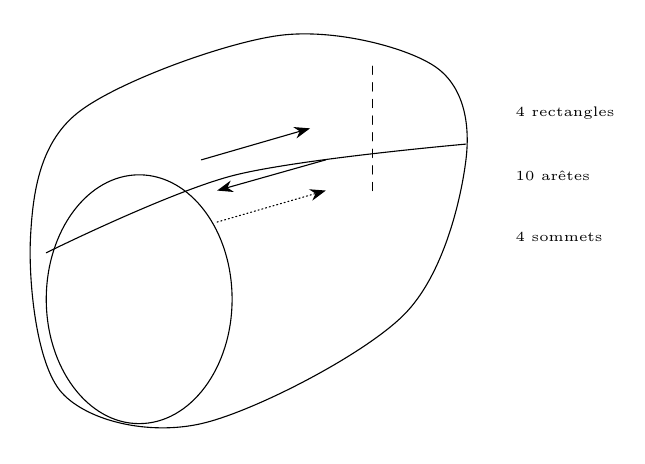
\begin{tikzpicture}[x=1mm,y=1mm,line cap=round,line join=round,font=\scriptsize]
\draw plot[smooth cycle, tension=0.55] coordinates {(9.2,-31.5) (15.1,-15.8) (40.8,-5.9) (60.5,-9.8) (64.5,-21.7) (56.6,-41.4) (30.9,-55.2) (13.2,-51.3)};
\draw plot[smooth, tension=0.55] coordinates {(11.2,-33.5) (34.9,-23.7) (64.5,-19.7)};
\draw (23,-39.4) ellipse[x radius=11.8, y radius=15.8];
\draw[dashed] (52.6,-9.8) -- (52.6,-25.6);
\draw[-{Stealth[length=2mm]}] (30.9,-21.7) -- (44.7,-17.7);
\draw[-{Stealth[length=2mm]}] (46.7,-21.7) -- (32.9,-25.6);
\draw[densely dotted,-{Stealth[length=2mm]}] (32.9,-29.6) -- (46.7,-25.6);
\node[inner sep=1pt,anchor=west] at (70.4,-15.8) {\tiny 4 rectangles};
\node[inner sep=1pt,anchor=west] at (70.4,-23.7) {\tiny 10 ar\^etes};
\node[inner sep=1pt,anchor=west] at (70.4,-31.5) {\tiny 4 sommets};
\end{tikzpicture}
\end{document}
